\chapter{Resultados}

Os resultados esperados, descritos no plano de atividades \citeonline{PlanoAtividades}, foram alcançados de forma satisfatória durante o desenvolvimento do trabalho. A seguir, são apresentados os resultados obtidos:

Compreensão detalhada das especificações do W3C-WoT: Foi realizada uma análise abrangente das especificações do W3C-WoT, resultando em uma compreensão aprofundada dos principais conceitos e requisitos para a implementação do WoTPy. Isso permitiu a correta e eficiente implementação do \textit{gateway}, seguindo os padrões estabelecidos pelo consórcio.

Seleção e domínio das bibliotecas e ferramentas adequadas: Foram selecionadas as bibliotecas e ferramentas mais adequadas para o desenvolvimento do WoTPy, levando em consideração a sua compatibilidade com os protocolos de comunicação necessários e a facilidade de integração com outros projetos IoT. O domínio dessas ferramentas foi crucial para o sucesso do trabalho.

Resolução dos problemas de instalação do WoTPy: Foram identificados e solucionados os problemas de instalação do WoTPy, resultando em um processo simplificado e eficiente para implantar e configurar o \textit{gateway} em diferentes ambientes e sistemas operacionais. Isso facilitou a adoção do WoTPy por parte dos desenvolvedores e usuários finais, garantindo uma experiência mais fluida.

Validação das contribuições por meio de testes: Um conjunto abrangente de testes foi realizado para validar as contribuições feitas ao WoTPy. Esses testes garantiram a qualidade e a funcionalidade do \textit{gateway}, verificando sua conformidade com os requisitos e sua capacidade de lidar com diferentes casos de uso.

Desenvolvimento de exemplos de uso e documentação detalhada: Foi criado um exemplo prático de uso do WoTPy, demonstrando sua aplicabilidade em cenário de IoT. Além disso, uma documentação detalhada foi elaborada, fornecendo orientações claras e recursos auxiliares para facilitar a implementação do WoTPy em projetos IoT. Isso contribuiu para a disseminação e adoção do \textit{gateway} pela comunidade.

\section{Especificações do W3C-WoT}

O Web das Coias (WoT) é uma iniciativa do \textit{World Wide Web Consortium} (W3C) que busca estabelecer uma estrutura para conectar dispositivos e serviços na Internet das Coisas (IoT). O objetivo do WoT é permitir a interoperabilidade entre esses dispositivos, facilitando a comunicação e a integração padronizadas.

O W3C desenvolveu várias especificações que abordam diferentes aspectos do WoT. Essas especificações são fundamentais para a implementação e adoção do WoT, proporcionando diretrizes para descrever as características das Coisas (\textit{Things}), definir interfaces de rede, realizar a descoberta de Coisas, implementar a lógica de aplicação e garantir a segurança e a privacidade dos sistemas WoT.

\begin{itemize}
    \item Descrição de Coisas (\textit{Thing Description}) \citeonline{TD} define um formato de dados legível por máquina para descrever os metadados e as interfaces de rede das Coisas. Ela fornece uma base sólida para a interoperabilidade entre as Coisas e a \textit{Web}.
    \item Modelos de Vinculação (\textit{Binding Templates}) \citeonline{WoTBinding} oferecem orientações sobre como definir interfaces de rede em Coisas para protocolos específicos e ecossistemas de IoT. Esses modelos são úteis para garantir a compatibilidade e a integração de diferentes sistemas.
    \item Descoberta (\textit{Discovery}) \citeonline{WoTDiscovery} define um mecanismo de distribuição de metadados das Coisas. Ela permite a localização e o acesso a informações detalhadas sobre as Coisas, facilitando a descoberta e a integração de dispositivos na rede.
    \item Modelos de Vinculação (\textit{Scripting API}) \citeonline{WoTScripting} possibilita a implementação da lógica de aplicação das Coisas utilizando uma API JavaScript comum. Isso simplifica o desenvolvimento de aplicativos IoT e promove a portabilidade entre fornecedores e dispositivos.
    \item Diretrizes de Segurança e Privacidade (\textit{Security and Privacy Guidelines}) \citeonline{WoTSecurity} oferecem orientações para a implementação segura das Coisas e discutem questões relacionadas à segurança e à privacidade nos sistemas WoT. Essas diretrizes são importantes para proteger os dispositivos e os dados sensíveis envolvidos nas redes WoT.
\end{itemize}

\subsection{Descrição de Coisas}

A Descrição de Coisas, é um formato de dados legível por máquina que descreve os metadados e as interfaces de rede das Coisas na Web das Coisas. Essa especificação, desenvolvida pelo W3C, fornece uma base sólida para promover a interoperabilidade entre as Things e a Web.

Através do WoT Thing Description, é possível descrever as características, propriedades, funcionalidades e interfaces de uma Thing de forma estruturada e padronizada. Essa descrição inclui informações detalhadas sobre como interagir com a Thing, como acessar seus recursos e como interpretar os dados que ela oferece.

Ao utilizar o formato de Descrição de Coisas WoT, torna-se mais fácil para diferentes dispositivos e sistemas compreenderem as capacidades e os requisitos de uma Thing específica. Isso possibilita a criação de aplicações e serviços que possam interagir de forma transparente com uma ampla variedade de Things, independentemente do fabricante ou da tecnologia subjacente.

A interoperabilidade é um aspecto fundamental na Web das Coisas, pois permite que as Things se comuniquem e interajam de maneira eficiente, facilitando a integração e a criação de soluções inovadoras. O WoT Thing Description desempenha um papel crucial nesse contexto, ao estabelecer uma linguagem comum para descrever as características das Things e ao promover a padronização na forma como essas informações são compartilhadas.

\subsection{Modelos de Vinculação}

Os Modelos de Vinculação, são diretrizes que oferecem orientações sobre como definir interfaces de rede em Coisas para protocolos específicos e ecossistemas de IoT. Esses modelos são extremamente úteis para garantir a compatibilidade e a integração entre diferentes sistemas.

Cada protocolo de comunicação utilizado na Web das Coisas possui suas próprias especificidades e requisitos. Os WoT Binding Templates fornecem um conjunto de instruções e recomendações para mapear as funcionalidades e os recursos de uma Thing em um formato compatível com um determinado protocolo.

Ao utilizar os WoT Binding Templates, os desenvolvedores podem criar interfaces de rede para suas Things que são consistentes com as exigências e os padrões dos protocolos específicos. Isso facilita a comunicação e a interação entre as Things e os sistemas que utilizam esses protocolos, garantindo uma maior interoperabilidade e uma integração mais suave.

Além disso, os WoT Binding Templates ajudam a promover a reutilização de código e a padronização na implementação das interfaces de rede. Ao seguir essas orientações, os desenvolvedores podem garantir que suas Things sejam facilmente integradas a ecossistemas de IoT existentes, evitando a necessidade de desenvolver soluções personalizadas para cada protocolo.

A utilização dos WoT Binding Templates também contribui para a escalabilidade e a flexibilidade dos sistemas de IoT. Como esses modelos oferecem uma estrutura padronizada para a definição de interfaces de rede, é mais fácil adicionar novas Things ao ecossistema e integrá-las com os sistemas existentes. Isso promove a expansão dos ecossistemas de IoT e facilita o desenvolvimento de soluções mais abrangentes e interconectadas.

\subsection{Descoberta WoT}

A Descoberta WoT, é um mecanismo que define a distribuição de metadados das Things na Web das Coisas. Essa especificação, desenvolvida pelo W3C, permite a localização e o acesso a informações detalhadas sobre as Things, facilitando a descoberta e a integração de dispositivos na rede.

A Descoberta WoT desempenha um papel fundamental na Web das Coisas, pois permite que os dispositivos IoT sejam encontrados e identificados de forma eficiente. Isso é especialmente importante em ambientes onde há uma grande quantidade de Things interconectadas, tornando a descoberta manual desses dispositivos inviável.

Ao utilizar o mecanismo de Descoberta WoT, é possível obter metadados sobre as Things, como suas funcionalidades, propriedades, interfaces de rede e outros atributos relevantes. Essas informações detalhadas permitem que os desenvolvedores e os sistemas de IoT identifiquem as Things que são relevantes para suas necessidades específicas.

Além disso, a Descoberta WoT possibilita a integração de dispositivos de diferentes fabricantes e tecnologias. Por meio da distribuição de metadados padronizados, os sistemas de IoT podem identificar e interagir com as Things de forma consistente, independentemente de suas características individuais.

A Descoberta WoT também contribui para a escalabilidade e a flexibilidade dos sistemas de IoT. Com a capacidade de localizar e acessar informações detalhadas sobre as Things, é mais fácil adicionar novos dispositivos à rede e integrá-los com os sistemas existentes. Isso promove a expansão dos ecossistemas de IoT e facilita o desenvolvimento de soluções mais abrangentes e interconectadas.

\subsection{API de Scripting WoT}

A API de Scripting WoT, é uma especificação que possibilita a implementação da lógica de aplicação das Things utilizando uma API JavaScript comum. Essa abordagem simplifica o desenvolvimento de aplicativos IoT e promove a portabilidade entre fornecedores e dispositivos.

Ao utilizar a WoT Scripting API, os desenvolvedores podem escrever o código de lógica de aplicação das Things em JavaScript, uma linguagem amplamente adotada e conhecida por sua flexibilidade e facilidade de uso. Isso elimina a necessidade de aprender linguagens de programação específicas de cada dispositivo ou fornecedor, tornando o processo de desenvolvimento mais eficiente e acessível.

A API de Scripting WoT fornece um conjunto de funcionalidades e métodos que permitem interagir com as Things, acessar seus recursos, enviar comandos e receber dados. Essa abordagem simplifica a implementação da lógica de negócios e a integração com outros componentes do sistema.

Além disso, a utilização da WoT Scripting API promove a portabilidade entre fornecedores e dispositivos IoT. Como a API é baseada em JavaScript, um padrão amplamente suportado, os aplicativos desenvolvidos com essa abordagem podem ser executados em diferentes dispositivos e plataformas, independentemente do fabricante.

Essa portabilidade é especialmente valiosa em cenários de IoT, onde há uma diversidade de dispositivos e fornecedores. Com a WoT Scripting API, é possível desenvolver aplicativos que podem ser implantados em uma ampla variedade de dispositivos IoT, reduzindo a dependência de fornecedores específicos e oferecendo mais flexibilidade aos desenvolvedores.

\subsection{Diretrizes de Segurança e Privacidade WoT}

As Diretrizes de Segurança e Privacidade WoT, são um conjunto de orientações que oferecem diretrizes para a implementação segura das Things e abordam questões relacionadas à segurança e privacidade nos sistemas WoT. Essas diretrizes são de extrema importância para proteger os dispositivos e os dados sensíveis envolvidos nas redes WoT.

A segurança e a privacidade são considerações críticas na Web das Coisas, pois os dispositivos IoT estão cada vez mais presentes em nosso cotidiano e lidam com uma grande quantidade de dados sensíveis. As WoT Security and Privacy Guidelines fornecem recomendações e melhores práticas para garantir a integridade, confidencialidade e disponibilidade dos dispositivos e dos dados na rede WoT.

Essas diretrizes abrangem uma variedade de aspectos de segurança, incluindo autenticação, autorização, criptografia, gerenciamento de chaves, proteção contra ataques e privacidade dos dados. Elas ajudam os desenvolvedores a identificar e implementar medidas de segurança apropriadas em suas Things, mitigando os riscos de exposição a ameaças e violações de privacidade.

Ao seguir as WoT Security and Privacy Guidelines, os desenvolvedores podem adotar práticas de segurança eficazes desde o design até a implementação das Things. Isso inclui a utilização de criptografia adequada para proteger a comunicação entre as Things, a implementação de mecanismos de autenticação robustos para garantir a identidade dos dispositivos e a adoção de políticas de privacidade que respeitem os direitos dos usuários.

Além disso, as diretrizes também incentivam a manutenção contínua da segurança e privacidade dos dispositivos e sistemas WoT, por meio de monitoramento, atualizações de segurança e resposta efetiva a incidentes. Isso é fundamental para garantir que os dispositivos IoT permaneçam protegidos ao longo do tempo, considerando a constante evolução das ameaças cibernéticas.

\section{Dependências do W3C-WoTPy}

O arquivo ''setup.py'' \citeonline{gitwotpy:setup} é responsável por definir as dependências necessárias para a execução da biblioteca WotPy, conforme especificado pelo \textit{World Wide Web Consortium} \cite{Architecture}. Essas dependências podem ser agrupadas em duas categorias: as obrigatórias e as opcionais.

Entre as principais dependências obrigatórias definidas no arquivo setup.py, estão:

\begin{itemize}
    \item tornado: uma biblioteca assíncrona utilizada para criar aplicativos web em Python. É empregada pela WotPy para estabelecer servidores HTTP e WebSocket.
    \item jsonschema: uma biblioteca que valida esquemas JSON e os dados JSON correspondentes. A WotPy utiliza essa biblioteca para validar as descrições de coisa (Thing Descriptions) recebidas e geradas.
    \item six: uma biblioteca que possibilita escrever código Python compatível tanto com a versão 2 quanto com a versão 3. A WotPy se beneficia dessa biblioteca para garantir a compatibilidade entre as duas versões do Python.
    \item rx: uma biblioteca de programação reativa que permite escrever código que responde assincronamente a mudanças de estado. É utilizada pela WotPy para suportar a API WoT Scripting e as interações com propriedades e eventos observáveis.
    \item python-slugify: uma biblioteca que converte strings para "slug", um formato de texto que utiliza apenas caracteres ASCII, números e traços. A WotPy utiliza essa biblioteca para criar identificadores únicos para as coisas.
\end{itemize}

Além dessas dependências obrigatórias, existem algumas dependências opcionais que a WotPy utiliza se estiverem disponíveis no sistema:

\begin{itemize}
    \item aiocoap: uma biblioteca Python para o protocolo de transferência de dados Constrained Application Protocol (CoAP), utilizada pela WotPy para suportar o protocolo CoAP.
    \item hbmqtt: uma biblioteca Python para implementar o protocolo Message Queue Telemetry Transport (MQTT), utilizada pela WotPy para suportar o protocolo MQTT.
    \item websockets: uma biblioteca Python para suportar a comunicação via WebSocket, utilizada pela WotPy para suportar o protocolo WebSocket.
    \item zeroconf: uma biblioteca Python para suportar o protocolo DNS Service Discovery (DNS-SD), utilizada pela WotPy para descobrir serviços e dispositivos na rede.
\end{itemize}

Essas dependências são verificadas em tempo de execução e adicionadas ao conjunto de dependências da biblioteca WotPy, caso estejam disponíveis no sistema.

\section{Resolução dos Problemas e Validação}

Este relatório aborda os problemas encontrados durante a execução e construção do projeto WotPy, disponível no GitHub \cite{gitwotpy:2022}. Inicialmente, foi realizado um \textit{fork} do projeto WotPy e o repositório \citeonline{gitwotpy:2023} foi clonado para o computador. 

\subsection{Construção do Projeto com Docker}

Ao tentar construir o projeto utilizando o ''\textit{docker build .}'', deparou-se com um erro relacionado à versão do ''pacote \textit{numpy}''. A mensagem de erro está descrito neste arquivo \cite{gitwotpy:cpd}.

Para solucionar esse problema, foi tentada inicialmente a alteração da versão do Python no arquivo ''\textit{Dockerfile}'' \cite{gitwotpy:v1}.

Posteriormente, optou-se por utilizar a versão original do Python (3.7) e, no arquivo ''examples/benchmark/requirements.txt'', foi revertida a versão modificada pelo ''dependabot[bot]'' \cite{gitwotpy:bot, gitwotpy:v2}.

Por fim, a solução adotada foi remover a inclusão das dependências do diretório ''/examples/benchmark'' no ''\textit{Dockerfile}'', mantendo a modificação anterior \cite{gitwotpy:v5}. Essa decisão foi tomada considerando que o exemplo do ''\textit{benchmark}'' não seria utilizado no projeto, e, portanto, as dependências relacionadas a ele não seriam necessárias.

\subsection{Execução dos Testes}

A execução dos testes do WoTPy foi iniciada com o seguinte comando''\textit{./pytest-docker-all.sh}''. Após a construção, foi identificado o erro descrito neste arquivo \citeonline{gitwotpy:et}. Para lidar com esse problema, o arquivo setup.py foi editado \cite{gitwotpy:v1}.

Dessa forma, o WoTPy pôde ser construído corretamente utilizando o Docker e passou nos testes propostos no ''pytest-docker-all.sh'.

\section{Desenvolvimento do Exemplo de Uso}

O exemplo demonstra a transmissão de dados do sensor UV de um microcontrolador ESP32 para um servidor Web of Things (WoT) via protocolo HTTP. O projeto utiliza a biblioteca WoTPy para criação do servidor e interações com o WoT, e o microcontrolador ESP32 emparelhado com um sensor UV ML8511.

Dois principais arquivos de código compõem este projeto: server.py e main.py. O arquivo server.py configura o servidor WoT, expõe um Thing que representa o sensor UV, e define \textit{handlers} customizados para leitura e gravação dos dados do sensor UV. O main.py, rodando no ESP32, periodicamente lê os dados do sensor UV e os envia para o servidor WoT usando requisições HTTP.

Este projeto serve como um exemplo base de integração de dispositivos IoT com princípios do WoT, facilitando a comunicação e a interoperabilidade entre dispositivos e aplicações dentro de um ecossistema de IoT.

\subsection{Protocolo de Comunicação}

A situação envolve um dispositivo ESP32 equipado com um sensor ML8511 (sensor UV) atuando como cliente, enquanto um computador atua como servidor utilizando a biblioteca WoTPy.

A comunicação entre o cliente ESP32 e o servidor Web of Things (WoT) é estabelecida por meio do protocolo HTTP, sendo uma escolha adequada para esse contexto. O uso do protocolo HTTP apresenta diversas vantagens que tornam essa abordagem viável e eficiente para o projeto em questão.

Uma das razões para a escolha do protocolo HTTP é a familiaridade do autor com essa tecnologia. Essa familiaridade agiliza o processo de desenvolvimento, evitando a necessidade de aprender um novo protocolo e me permitindo aproveitar a experiência prévia nessa área.

Além disso, o HTTP é amplamente utilizado na web e conta com recursos de implementação disponíveis para diferentes plataformas e linguagens de programação, incluindo o \textit{MicroPython} utilizado no ESP32. Existem bibliotecas e ferramentas prontamente disponíveis que facilitam a implementação da comunicação HTTP, possibilitando um desenvolvimento mais eficiente e eficaz.

O HTTP também oferece suporte a uma variedade de métodos de solicitação, como GET, POST, PUT e DELETE, permitindo que o cliente ESP32 envie solicitações para ler, gravar e excluir dados no servidor WoT. Essa flexibilidade é fundamental para a interação entre o cliente e o servidor, possibilitando a troca de informações necessárias para o correto funcionamento do sistema WoT.

\subsection{Cliente Web of Thing (WoT)}

O código ''main.py'' \citeonline{gitwotpy:main} implementa um cliente Web of Things (WoT) no dispositivo ESP32, permitindo a interação com sensores e o envio dos dados para um servidor WoT. O cliente WoT é responsável por buscar informações dos sensores e controlar as funcionalidades dos dispositivos conectados de maneira padronizada e interoperável.

O cliente WoT utiliza o protocolo HTTP para se comunicar com o servidor WoT. No código, é feito uso da biblioteca \textit{urequests} para realizar solicitações HTTP PUT ao servidor. Essas solicitações enviam os dados dos sensores em formato JSON para o servidor WoT, permitindo que os dados sejam armazenados e acessados pelos usuários.

O código define os sensores utilizados no dispositivo ESP32, como o sensor de UV, e suas configurações. Cada sensor possui uma identificação única e é associado a uma descrição no formato de Thing Description (TD). A TD contém informações sobre o sensor, como os links de acesso aos dados no servidor WoT.

A função \textit{send\_sensor\_data} é responsável por enviar os dados dos sensores para o servidor WoT. Ela recebe como parâmetros a identificação do sensor, o tipo de sensor, o URL de acesso aos dados na TD e os dados a serem enviados. A função realiza uma solicitação HTTP PUT ao URL especificado, enviando os dados em formato JSON. Se a solicitação for bem-sucedida, uma mensagem de sucesso é exibida. Caso contrário, uma mensagem de falha é exibida juntamente com o código de status da resposta.

No loop principal main(), os valores dos sensores são lidos periodicamente. A cada iteração do loop, os dados dos sensores são obtidos e enviados para o servidor WoT utilizando a função \textit{send\_sensor\_data}. Esse processo permite que os dados dos sensores sejam atualizados no servidor WoT em tempo real, possibilitando que os usuários acessem e utilizem essas informações de forma padronizada, como é representado na figura \ref{fig:sequencia}.

\subsection{Servidor Web of Things (WoT)}

O servidor Web of Things (WoT) é uma peça fundamental na arquitetura WoT, pois é responsável por expor os dispositivos conectados e suas funcionalidades para que possam ser descobertos e interagidos pelos clientes. O servidor WoT atua como uma ponte entre os dispositivos da Internet das Coisas (IoT) e os aplicativos e serviços que desejam acessá-los.

O código server.py \citeonline{gitwotpy:server} implementa um servidor Web of Things (WoT) que expõe uma Thing (dispositivo) responsável por fornecer os valores de um sensor de UV. O servidor WoT permite a descoberta e interação com a Thing por meio de solicitações HTTP padronizadas.

O servidor WoT utiliza a biblioteca Tornado e o protocolo HTTP para receber solicitações dos clientes e responder de acordo com as interações definidas na descrição da Thing. A Thing é definida por uma descrição no formato de um documento JSON, que especifica suas propriedades e comportamentos.

No código, é criado um HTTP server na porta especificada (HTTP\_PORT) e um Servient, que é uma instância responsável por gerenciar os recursos WoT. A descrição da Thing é definida, contendo o identificador (ID\_THING) e as propriedades, como o sensor de UV.

Para cada propriedade da Thing, como o sensor de UV, são definidos os manipuladores de leitura (read\_uv) e escrita (write\_uv). O manipulador de leitura é responsável por retornar o valor atual do sensor quando solicitado pelo cliente. O manipulador de escrita é responsável por atualizar o valor do sensor quando recebido uma solicitação de escrita do cliente.

Ao iniciar o servidor, é criado o objeto WoT, e a Thing é produzida com base na descrição. Em seguida, os manipuladores de leitura e escrita são associados à propriedade correspondente na Thing. Isso permite que o servidor WoT responda às solicitações de leitura e escrita para o sensor de UV.

Por fim, a Thing é exposta e o servidor inicia seu loop de eventos, aguardando as solicitações dos clientes e respondendo de acordo com as interações definidas, como é representado na figura \ref{fig:sequencia}.

\begin{figure}
    \centering
    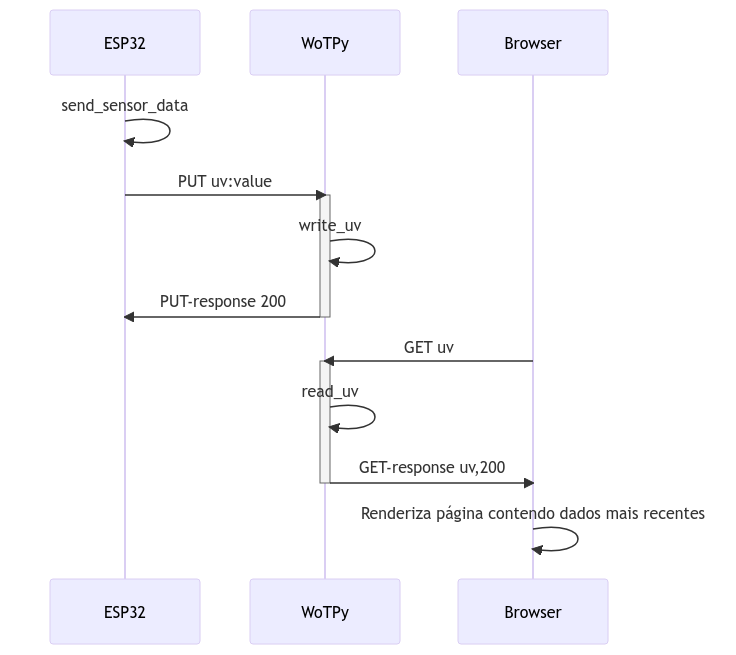
\includegraphics[scale=0.6]{figs/sequencia.png}
    \caption{O dispositivo (ESP32) executa um loop que, a cada 5 segundos executa a função send\_sensor\_data. Esta função envia uma requisição PUT para o servidor (WoTPy). Em resposta a essa requisição o servidor executa o handler (função) write\_uv que contém o envio da resposta. Um usuário pode acessar a informação no servidor através do Browser. Entrar a URL na barra de endereços do Browser o faz enviar ao servidor uma requisição GET. Em resposta à requisição o servidor executa o handler (função) read\_uv, que contém o envio da resposta - no caso, o valor de uv mais recente. O Browser recebe essa informação e renderiza a página contendo a informação.}
    \label{fig:sequencia}
\end{figure}

